\section{Component Design} \label{sec:componentdesign}

In this section the component design theory will be introduced and elaborated.
This theory will be utilized in the following section where the component design for the system will be presented.
%Anna: evt fjerne sætningen ovenfor da det virker til at være en gentagelse af den første

\subsection{Components}


\subsection{System design} \label{sec:systemdesign}

In relation to the ASP.NET MVC pattern there are immediate similarities to the component design theory in \cref{archicomponents}.
There can among other be drawn parallels between the \textit{model} component and the \textit{model} classes in the MVC pattern.
The possible parallels are listed in the table below.
%There can likewise be drawn parallels between the \textit{functionality} component and \textit{controller} classes, and \textit{interface} component and the \textit{view} in the MVC pattern.
%The parallels are listed as seen in the table below:
\begin{table}
	\centering
	\begin{tabular}{| c | c | }
	\hline
	\textbf{Components} & \textbf{MVC Pattern} \\
	\hline
	Model & Model \& EF Core \\
	\hline
	Functionality & Controller \\
	\hline
	Interface & View \\
	\hline
\end{tabular}
\caption{{\color{red}indsæt caption tekst}}\label{tab:PatternParallels}
\end{table}

As written in the component design theory the model components should seek to solve the problem of the problem domain.
%Anna: enten henvis til specifikke definition hvis sådan en eksisterer ellers henvis til afsnittet.
%Anna: Mener vi virkeligt "problem og the problem domain"
The model component in the MVC pattern is likewise going to contain the classes and objects that seeks to solve the problem domain through meeting the requirements written in {\color{red}section xx}.
The model component in the implementation is among other classes going to contain \textit{documents, users, departments, versions, approvals} and \textit{read statuses}.
The arguments for including these classes can be seen in \cref{sec:classdiagram}.
The database in form of EF Core is also included in the model component as this in part also seeks to solve the problem domain.
%Anna: Vi hrar endnu ikke introdyuceret denne forkortelse i brødteksten(EF core)

As written in the component design theory the responsibilty of the functionality is to provide the actor a means to access the model component.
%Anna: Henvis til afsnitet
The controller component in the MVC pattern does this by communicating between the model component and the view component.
The controllers retrieves data from the database and both methods and objects from the models.
Hereafter,it links these to the view.

The responsibility of the interface component is the handle the interaction between the users and the functionality.
This is done through the view model in the MVC pattern as the interface is handled in big part due to HTML, CSS and JavaScript.
These are what determines what the actors sees and what they can interact with.

\subsection{Component layers}
In relation to the theory written in \cref{archicomponents} the components can be designed in layers to describe their responsibilities and relation to each other.
The components in the MVC pattern with EF Core included can also be designed with the layered architecture in mind.
To give an overview and understanding of the architecture and design a simple component layer design can be seen in the figure below:
%Anna: synes den sidste sætning bliver en smule kringlet

\begin{figure}[H]
	\centering
	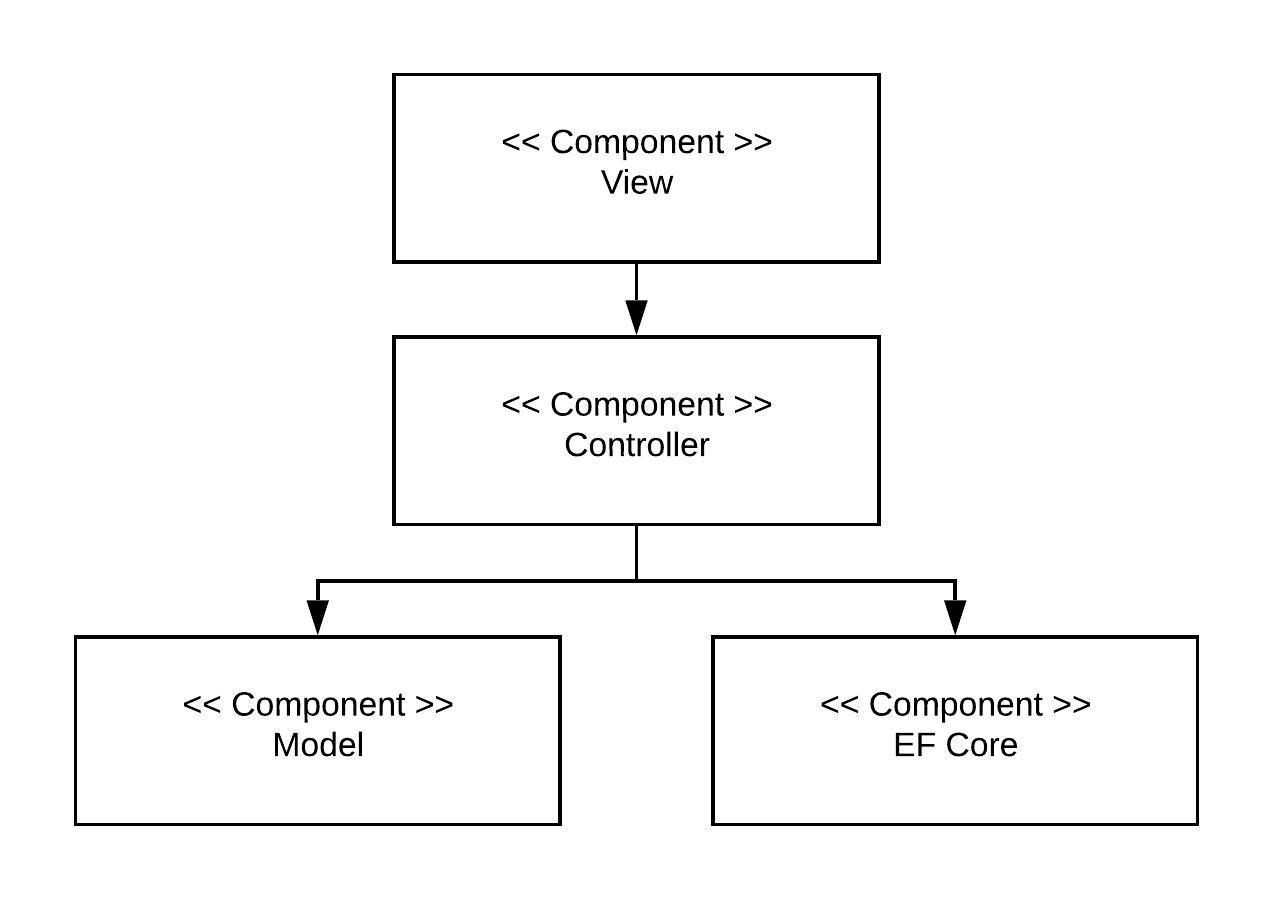
\includegraphics[width=0.7\textwidth]{billeder/simplecomponents.jpeg}
	\caption{Simple component layer design}\label{fig:SimpleComponent}
\end{figure}

View, controller, model, and EF Core are thus the main components layers that can be found in the design, each with a well-defined responsibility.
Ideally the architecture is designed so that the view and model components do not have to interact with each other.
% Kilde? Det virker lidt suspekt at views og models ikke skal kunne snakke med hinanden
It is the intention that the controller is the link between these components, which is why it is placed in the middle of the layer components.
The main function of the controller is to link objects from the model component and data from the EF Core database and make these accessible for the view component.

%Anna: vil vove at påstå der ikke birde være et afsnit her
This will not always be the case as the ASP.NET Core MVC model is designed so that a view has a corresponding controller.
For example the document view will have a corresponding document controller.
The document view will eventually have to borrow objects and data from other models in the system, which means that the view will at times have to bypass the controller component to communicate with the model component.

Subsystems can be explored from the main components, which e.g. are the interface system and its underlying technologies.
These are HTML, CSS, JavaScript and razor.
The model component has two main parts which are the model classes from the MVC pattern and the EF Core database system.
These two are defined as separate components which share similar responsibilities in the model component.

%Anna: Vil igen vove at påstå det ikke burde være et afsnit her
These components their relations with each other, and their underlying sub components can be seen in the complex version of the layer design below:
\todo[inline]{Fix tabellen efter Lu's kommentarer}

\begin{figure}[H]
	\centering
	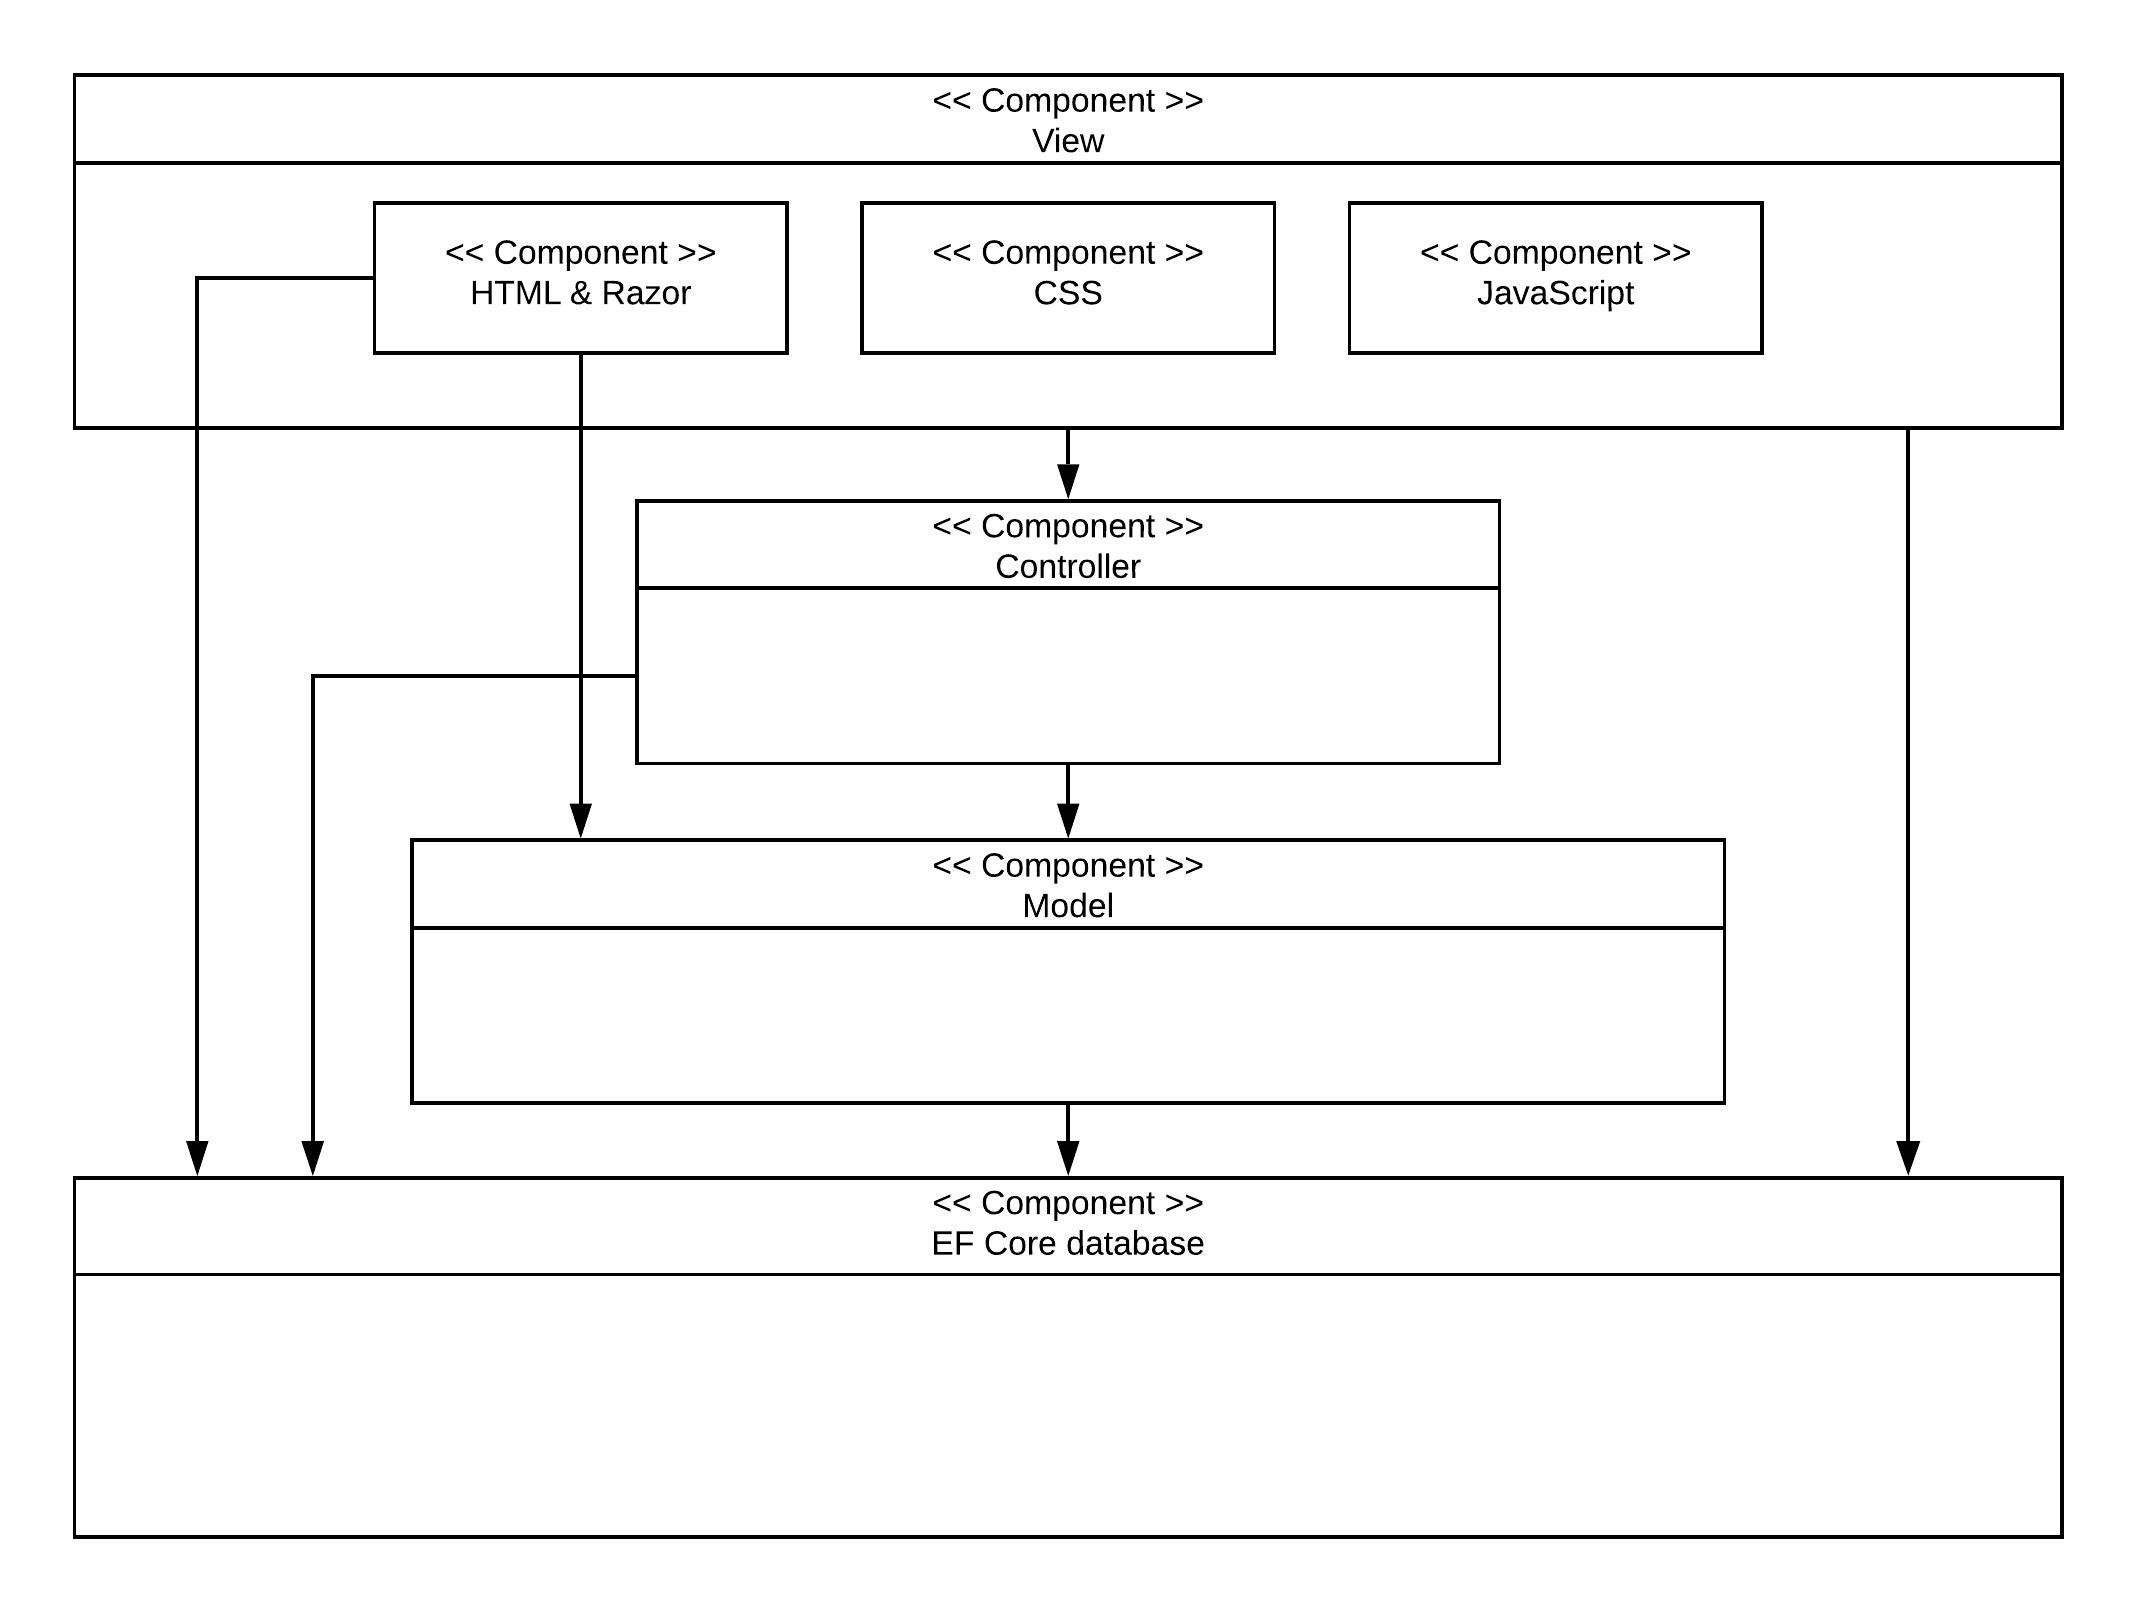
\includegraphics[width=1\textwidth]{billeder/complexcomponents.jpeg}
	\caption{Complex component layer design}
\end{figure}

Ideally the design would have \textit{closed-relaxed} architecture as the components would only be able to access layers adjacent to them.
In this design the design would be \textit{relaxed} as the controller would have access to both the view and the model components.
As it is though the design has an \textit{open-relaxed} architecture as the view component occasionally has access to the model component.
%Anna: Kan godt tænkes de to sidste sætninger trænger til en omskrivning

In the final design there will be several classes included within each of the components.
Each of the main classes in the model component will have a corresponding controller and view in relation to it.
For example the document class in the model component will have a corresponding database in EF Core as well as a corresponding controller and view.
Here the documents object is within the model component and the documents data will be stored in the database.
A corresponding controller, which mainly handles the document class, ensures that the class and database are accessible for the actor.
The corresponding view ensures that the actor is able to see and interact with the document classes and database.
